% ****** Start of file apssamp.tex ******
%
%   This file is part of the APS files in the REVTeX 4.1 distribution.
%   Version 4.1r of REVTeX, August 2010
%
%   Copyright (c) 2009, 2010 The American Physical Society.
%
%   See the REVTeX 4 README file for restrictions and more information.
%
% TeX'ing this file requires that you have AMS-LaTeX 2.0 installed
% as well as the rest of the prerequisites for REVTeX 4.1
%
% See the REVTeX 4 README file
% It also requires running BibTeX. The commands are as follows:
%
%  1)  latex apssamp.tex
%  2)  bibtex apssamp
%  3)  latex apssamp.tex
%  4)  latex apssamp.tex
%
\documentclass[%
 reprint,
%superscriptaddress,
%groupedaddress,
%unsortedaddress,
%runinaddress,
%frontmatterverbose, 
%preprint,
%showpacs,preprintnumbers,
%nofootinbib,
%nobibnotes,
%bibnotes,
 amsmath,amssymb,
 aps,
%pra,
%prb,
%rmp,
%prstab,
%prstper,
%floatfix,
]{revtex4-1}

\usepackage{graphicx}% Include figure files
\usepackage[utf8]{inputenc}
\usepackage{dcolumn}% Align table columns on decimal point
\usepackage{bm}% bold math
%\usepackage{hyperref}% add hypertext capabilities
%\usepackage[mathlines]{lineno}% Enable numbering of text and display math
%\linenumbers\relax % Commence numbering lines

%\usepackage[showframe,%Uncomment any one of the following lines to test 
%%scale=0.7, marginratio={1:1, 2:3}, ignoreall,% default settings
%%text={7in,10in},centering,
%%margin=1.5in,
%%total={6.5in,8.75in}, top=1.2in, left=0.9in, includefoot,
%%height=10in,a5paper,hmargin={3cm,0.8in},
%]{geometry}

\begin{document}

\preprint{APS/123-QED}

\title{Radiactividad}% Force line breaks with \\
\thanks{}%

\author{Jesus Prada}
 \email{jd.prada1760@uniandes.edu.co}
 \altaffiliation[Also at ]{Departamento de Física, Universidad de los Andes}%Lines break automatically or can be forced with \\
\author{Sergio Iv\'an Rey}%
 \email{si.rey1826@uniandes.edu.co}
\affiliation{%
 Departamento de Física, Universidad de los Andes
}%

\date{10/09/2015}% It is always \today, today,
             %  but any date may be explicitly specified

\begin{abstract}
En este experimento verificamos la naturaleza del comportamiento de la radiación ionizante por medio de diversos experimentos que caracterizaban cada cualidad particular de este fenómeno nuclear. Pudimos verificar la composición de radiación en términos de rayos $\alpha$, $\beta$ y $\gamma$ de diversas fuentes radiactivas teniendo en cuenta su poder de penetración sobre diferentes filtros. Especialmente verificamos que la radiación $\beta$ es cargada y de masa minúscula, mientras que la radiación $\gamma$ no tiene carga. Demostramos que el proceso estocástico de decaimiento radiativo es bien modelado por la distribución de Poisson. De esta manera pudimos deducir la varianza y el error de las mediciones sin tener muestras estadísticas significativas. Demostramos además con error de alrededor de 2\% que la intensidad de radiación decae con el cuadrado de la distancia a la fuente y como una ley exponencial con la distancia a la que penetra un material absorbente. Con el criterio del intervalo de confianza proporcionado por la varianza, pudimos demostrar la radiactividad o inactividad de diferentes elementos como rocas con trazas radiactivas y diversas sales. Además verificamos cuantitativamente la ley de decaimiento exponencial con el tiempo al medir el tiempo de actividad característico de una muestra de aire radiactivo.
\end{abstract}


\keywords{}%Use showkeys class option if keyword
                              %display desired
\maketitle

%\tableofcontents

\section{\label{sec:level1}Introducci\'on}

El descubrimiento de los elementos radiactivos por Pierre y Marie Curie a principios del siglo XX dio paso al desarrollo de la física nuclear, una oleada de nuevas tecnologías, el desarrollo de nuevas maneras de producción de energía y una especie de nueva revolución industrial. Por ello, el estudio de las fuentes radiactivas ha sido de mayor interés durante el último siglo para la ingeniería y las ciencias naturales en general, y por ello se ha desarrollado este experimento. El entendimiento de la radiactividad será de utilidad para el estudiante para desarrollar competencias en física nuclear y de partículas, como también proveerá de un entendimiento global de los fenómenos que acontecieron en el siglo XX.\\

La radiactividad es un fenómeno físico en el cual isótopos inestables de algunos átomos,  con el fin de alcanzar un estado más estable, pierden energía por medio de la emisión de ondas electromagnéticas o bien por la pérdida, de parte de sus núcleos, de partículas más pequeñas.\\

La radiactividad puede ser clasificada en dos categorías según la manera de emisión. Así pues, la radiactividad natural se produce cuando espontáneamente los átomos emiten energía en las formas anteriormente mencionadas para alcanzar un estado más estable.\\

En caso contrario, la radiactividad artificial o inducida ocurre cuando se libera energía al bombardear partículas pequeñas contra átomos inestables causando su ruptura, proceso cono cocido como fisión nuclear. EL proceso opuesto, conocido como fusión nuclear, es el de colisionar átomos pequeños para formar unos más grandes con el fin de liberar energía.\\

Por otra parte, dada su naturaleza de emisión, se puede catalogar la radiación en tres categorías diferentes:\\


-Radiación alfa ($ \alpha $): Es el flujo de partículas alfa, que consisten de dos neutrones con dos protones. En otras palabras, es la emisión de iones de $He^{2+}$. Este tipo de radiación es altamente ionizante pero muy poco penetrante y sólo se presenta cuando átomos con $A>100$ decaen para formar átomos más pequeños. La producción de una partícula alfa está dada por la ecuación:\\

\begin{equation}
	^{A}_{Z}X \to ^{A-4}_{Z-2}Y+\alpha
\end{equation}

-Radiación beta ($ \beta $): Consiste en el flujo de electrones ($ \beta - $), o de positrones ($ \beta + $). Esta radiación, en el primer caso el átomo debe tener un exceso de neutrones, así uno de éstos decaerá para formar un positrón, un electrón y un antineutrino, el cual es una partícula agregada a la ecuación por Fermi para soportar el balance energético y la conservación del número leptónico y bariónico; su existencia fue probada experimentalmente años después. Su reacción está dada por:\\

\begin{equation}
	n^0 \to p^{+} + e^{-} + \bar{\nu}
\end{equation}

El átomo al cual pertenece el neutrón cambia de la siguiente forma: \\

\begin{equation}
	^{A}_{Z}X \to ^{A}_{Z+1}Y + e^{-} + \bar{\nu}
\end{equation}

También puede ocurrir que el neutrón decaiga para producir un positrón y un neutrino, en cuyo caso el átomo cambia de la siguiente manera, esta radiación es conocida como beta positiva:\\

\begin{equation}
^{A}_{Z}X \to ^{A}_{Z+1}Y + e^{+} + \nu
\end{equation}

-Radiación Gamma ($ \gamma $): La radiación Gamma es la emisión de ondas electromagnéticas con longitud de onda muy corta. Se considera la radiación más peligrosa y penetrante, ya que usualmente se requiere de muros de hormigón de varios centímetros para detenerla. Esta radiación se produce cuando un átomo decae de un estado excitado a otro más estable, pero no pierde ninguna partícula. Así:\\

\begin{equation}
	^{A}_{Z}X^{\star} \to ^{A}_{Z}X + \gamma 
\end{equation}

Los diferentes tipos de radiación requieren así, diferentes tipos de barreras para ser detenidas y esto por lo general depende de la masa y la carga de la partícula emitida. Así, dado el gran tamaño de la partícula alfa, se requiere sólo una hoja de papel. Los electrones son significativamente más pequeños, y por lo tanto requerirán una lámina delgada de algún metal o unos centímetros de agua.\\


\section{\label{sec:level1}Montaje experimental}
\textit{Contador Geiger-Muller}\\
El dispositivo usado durante la práctica es un contador de Geiger-Muller. Éste es un dispositivo que sirve para medir la intensidad de la fuente radiactiva. El dispositivo consiste en un filamento conductor muy delgado dentro de un tubo metálico. Ambos están aislados por un gas inerte. De esta manera, cuando una partícula desprendida de un átomo que está en proceso de decaimiento, entra al detector e interactúa con el filamento, produce un impulso eléctrico cuya amplificación es audible. Esto se conoce como una cuenta. Así pues, a mayor cantidad de cuentas, mayor se considera que es la intensidad de la fuente radiactiva.\\

Durante esta práctica utilizamos este contador en diferentes configuraciones para medir la radiación emitida por diversas fuentes radiactivas y por el ambiente. En general posicionábamos el detector el dispositivo Geiger en frente de una fuente como se muestra en la figura \ref{fig:montaje}. Con ayuda de los soportes que se muestran en dicha figura podíamos variar la distancia entre el detector y la fuente además de su ángulo. Además de esto, las escalas estaban impresas en la mesa de trabajo, por lo cual, la toma de medidas era sencilla.\\

\begin{figure}[h!]
\centering
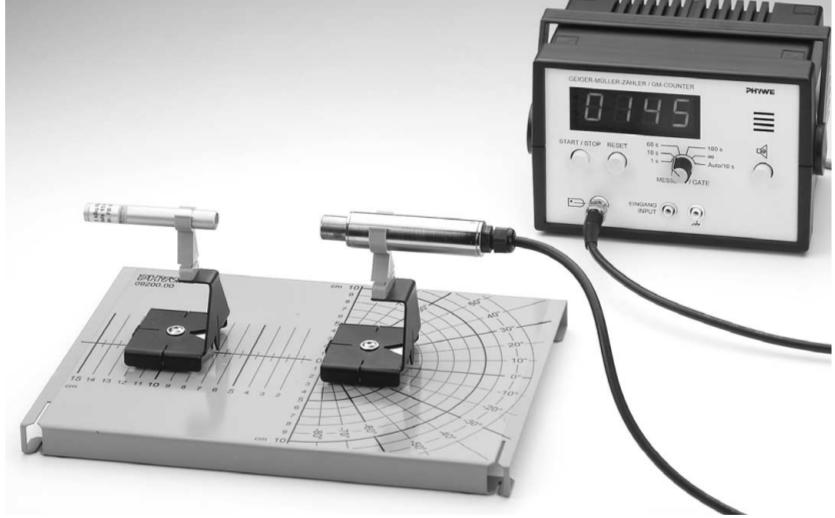
\includegraphics[width=1\linewidth]{montaje.jpg}
\caption{Montaje experimental general}
\label{fig:montaje}
\end{figure}

En el caso en que era preciso tomar conteos con filtros, se ponían filtros con ayuda de los soportes entre el detector y la fuente, como se muestra en la figura \ref{fig:montaje-filtros}. \\

\begin{figure}[h!]
\centering
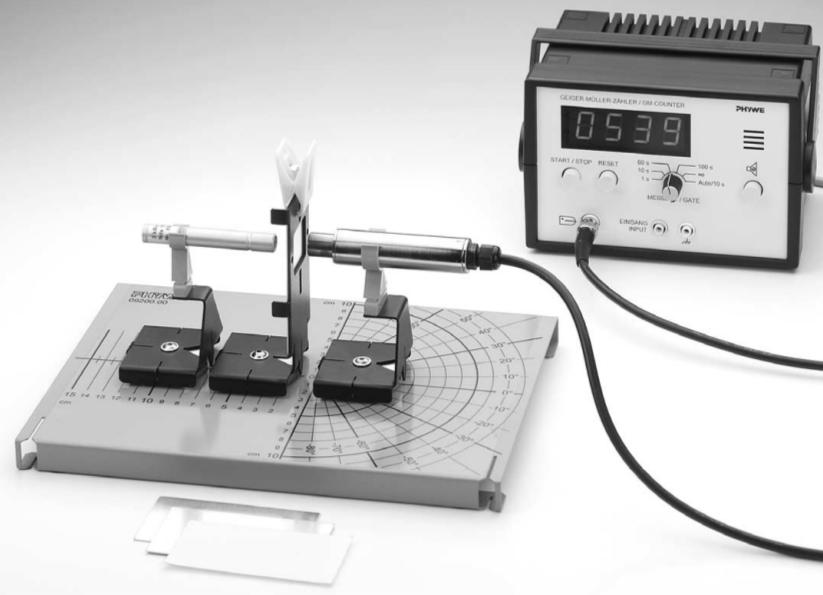
\includegraphics[width=1\linewidth]{montaje2.jpg}
\caption{Montaje experimental con filtros}
\label{fig:montaje-filtros}
\end{figure}

De la misma manera, en el caso en que verificamos el efecto del campo magnético sobre la radiación, lo que hicimos fue posicionar dos magnetos con polarización paralela en medio de la trayectoria de la radiación de la fuente al detector. Dichos magnetos eran posicionados con ayuda del soporte multifuncional proporcionado en el laboratorio. Un ejemplo de este montaje se puede apreciar en la figura \ref{fig:magnetico}.\\


\begin{figure}[h!]
\centering
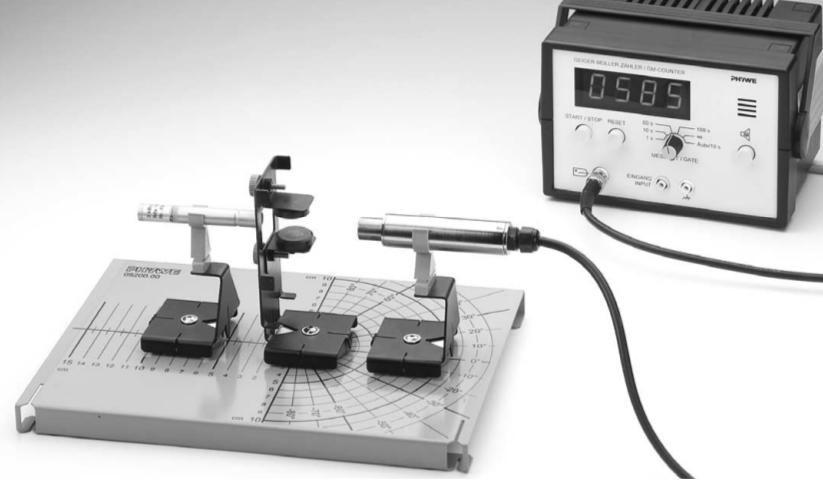
\includegraphics[width=1\linewidth]{magnetos2.jpg}
\caption{Montaje experimental con magnetos}
\label{fig:magnetico}
\end{figure}

En el caso especial en que medimos la radiactividad en una muestra de aire proveniente de una manta radiactiva, encerramos dicho aire con ayuda de una jeringa en un recipiente con apertura del mismo tamaño y forma del contador. Acto seguido tapamos el recipiente con el contador y empezamos a tomar medidas. Dicho montaje puede ser apreciado en la figura \ref{fig:airemontaje} .\\


\begin{figure}[h!]
\centering
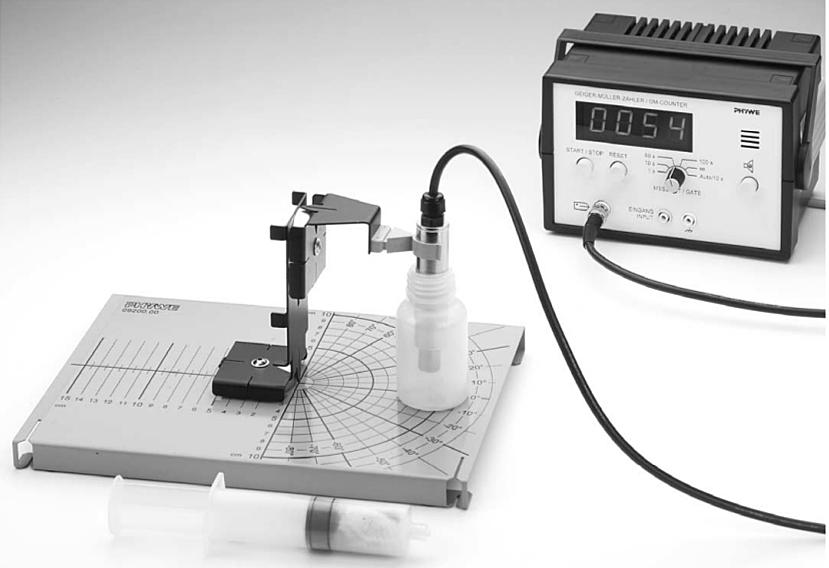
\includegraphics[width=1\linewidth]{aire.jpg}
\caption{Montaje experimental para una muestra de aire radiactivo}
\label{fig:airemontaje}
\end{figure}

En general, debido a que el detector Geiger era separado del su contador, unidos únicamente por un cable, ese experimento permitía mucha libertad de movimiento para poder configurar los montajes y realizar las mediciones.\\

\section{\label{sec:level1}Resultados y An\'alisis}

\subsection{\label{sec:level2}Radiación de fondo}
En este experimento medimos la radiación de fondo promedio. Tomamos 5 datos de 60 segundos cada uno, los cuales se encuentran registrados en la tabla \ref{table:fondo}.\\

\begin{table}[h!]
\centering
\begin{tabular}{|c|}
	\hline $ Conteo (\pm 1) $ \\ 
	\hline\hline
	27\\
	20\\
	16\\
	19\\
	24\\
	[1ex] 
 \hline
 \end{tabular} 
  \caption{Radiación ambiental}
\label{table:fondo} 
\end{table}

El objetivo de este experimento era verificar si se podía detectar radiación en ausencia de una muestra. Esta radiación detectada la llamamos radiación de ambiente y se debe a decaimientos espontáneos de isótopos radiactivos en la materia que nos rodea; a la radiación cósmica de fondo y a las muestras de radiación que se encontraban en mesas cercanas. Las muestras que se encontraban en dichas mesas variaban constantemente su ubicación y su nivel de radiactividad dependía de los experimentos que otros estuvieran haciendo, por lo cual era conveniente medir la radiación de fondo al realizar cada montaje.\\

Esta radiación de fondo tiene como promedio un valor de $21.2$ conteos por cada 10 segundos. En estas mediciones, debido al caracter probabilístico de su naturaleza, una buena medida del error es la desviación estándar. A lo largo de este informe escogemos la definición de error absoluto asociado a su medida como su desviación estándar. Esta medida, $\delta x = \sigma_x$ tiene un $68.27\%$ de confianza, es decir, cada medida tiene  $68.27\%$ de probabilidad de estar en el rango dado por dicho error. \\

En este caso, la media, incluyendo su error absoluto está dada por $C = 21.2 \pm 3.86\frac{cts}{10s}$. Esta medida de error, es cada vez más confiable entre más medidas tengamos, dado que la desviación estandar real asociada a la distribución de probabilidad del fenómeno se obtiene, por definición, sobre un número infinito de realizaciones de dicha distribución. Podemos ver la veracidad de este factor dado que en este caso obtuvimos un error relativo bastante grande para solo 5 medidas: $18.2\%$.\\

\subsection{\label{sec:level2}Variaciones} 
En este experimento verificamos la naturaleza estadística de la radiación al tomar 50 medidas de 10 segundos sobre una manta incandescente.\\

La distribución de probabilidad que mejor caracteriza el proceso estocástico de decaimientos radiactivos es la distribución de Poisson. Esta distribución tiene como característica que su varianza es igual a su promedio, y en términos de la desviación estándar: $\sigma_x^2 = \bar{x}$. Debido a que esta distribución es discreta, hacer cálculos de intervalos de confianza resulta difícil, sin embargo, podemos aproximar su forma de campana como una Gaussiana. En este sentido, se tiene que el $68.27\%$ de los datos estarán concentrados alrededor del promedio con radio igual a una desviación estándar. Si se escoje un radio de $2\sigma$, $95.45\%$ de los datos estarán concentrados en el intervalo, y si se tienen $3\sigma$ (el error absoluto definido para este informe), se tendrá una confianza del $99.73\%$.\\

Teniendo los anteriores datos en cuenta, se puede notar que el porcentaje de error debido a la definición $\delta x = \sigma_x$ está dado por $\epsilon = \frac{\sigma_x}{\bar{x}} = \frac{1}{\sqrt{\bar{x}}}$. Esto evidencia la importancia del tiempo en las medidas que tomamos, ya que si se toman conteos por un intervalo de tiempo mayor, el promedio será claramente mayor, y por tanto, el error relativo disminuirá. Además de esto, con esta propiedad es posible estimar el error asociado a una medida sin tener una muestra estadistica significativamente grande.\\


Sin más preámbulos, los datos obtenidos se encuentran consignados en la tabla \ref{table:variaciones} y un histograma donde se pueden apreciar claramente las características de una distribución de Poisson con baja resolución, se encuentra graficado en la figura \ref{fig:variaciones}.\\

\begin{table}[h!]
\centering
\begin{tabular}{|c|c|c|c|}
	\hline $ N^oMedicion $ & $Resultado(\pm 1)$ & $ N^oMedicion $ & $Resultado(\pm 1)$ \\ 
	\hline\hline
	1&65&26&66\\
	2&63&27&73\\
	3&57&28&60\\
	4&67&29&59\\
	5&67&30&82\\
	6&78&31&74\\
	7&67&32&72\\
	8&56&33&62\\
	9&78&34&66\\
	10&55&35&57\\
	11&80&36&75\\
	12&69&37&56\\
	13&61&38&79\\
	14&70&39&65\\
	15&68&40&68\\
	16&65&41&75\\
	17&69&42&67\\
	18&58&43&71\\
	19&71&44&73\\
	20&75&45&65\\
	21&61&46&69\\
	22&73&47&70\\
	23&54&48&64\\
	24&79&49&56\\
	25&64&50&64\\	
		[1ex] 
 \hline
 \end{tabular} 
  \caption{Variación estadística}
\label{table:variaciones} 
\end{table}


\begin{figure}[h!]
\centering
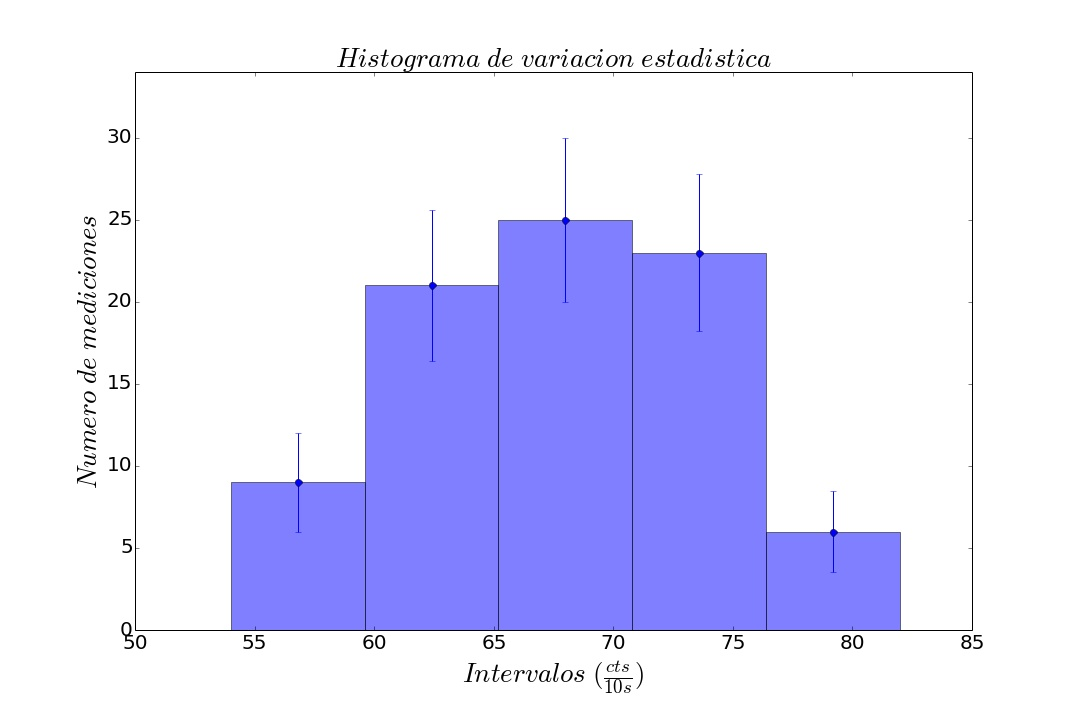
\includegraphics[width=1\linewidth]{variacion.jpg}
\caption{Histograma de los conteos medidos}
\label{fig:variaciones}
\end{figure}

En este experimento se obtuvo un promedio de 67.16 conteos cada 10 segundos, y una desviación estándar de    7.19 en las mismas unidades. Nótese que la raiz cuadrada del promedio debería ser igual a la desviación estándar si la distribución estudiada es de Poisson. En este caso dicha raiz es de 8.19, que comparada con el valor real, presenta un error de solo $12\%$, lo cual es bastante razonable para un análisis estadístico.\\

Ahora, al verificar el intervalo de confianza que provoca una desviación estándar, descubrimos que el $64\pm2\%$ de los datos se encontraban en dicho intervalo, lo cual muestra un error de 6.25\% con el valor esperado de $68\%$.\\

Los errores obtenidos en este montaje son naturales de la calidad estocástica de los procesos involucrados. En principio, para los análisis estadísticos siempre necesitaremos una cantidad infinita de mediciones para obtener conclusiones exactas. A pesar de dichos errores, pudimos identificar la distribución de probabilidad de las medidas como una distribución de Poisson.\\

\subsection{\label{sec:level2}Radiactividad en sales} 
En esta sección verificamos si las muestras de sales $CaCl$, $Cu_2SO_4$, $NaCl$, $KCl$ emitían radiación ionizante. Para ello medimos cuatro veces los conteos que provocaban en el contador Geiger duratnte 60 segundos, y los comparamos con la radiación del ambiente.\\

Los datos obtenidos se encuentran consignados en la tabla \ref{table:sales}.\\

\begin{table}[h!]
\centering
\begin{tabular}{|c|c|c|c|c|c|c|}
	\hline $ Muestra $ & \multicolumn{4}{c|}{$Resultado\ (\pm 1)$ } & $\bar{x}$& $\sigma_x$ \\ 
	\hline\hline
	CaCl2&28&22&21&22&23.25&2.77\\
	Cu2SO4&21&15&32&16&21.0&6.75\\
	KCl&43&41&44&34&40.5&3.91\\
	NaCl&25&23&23&16&21.75&3.42\\
	Ambiente&23&23&23&15&21.0&3.46\\
	[1ex] 
 \hline
 \end{tabular} 
  \caption{Radiación por diferentes muestras de sales}
\label{table:sales} 
\end{table}

De esta tabla, teniendo en cuenta las desviaciones estándares, se puede concluir el cloruro de potasio es claramente radiactivo ya que, teniendo en cuenta el error estadístico, su intervalo no cae en la radiación ambiente; el cloruro de calcio es posiblemente radiactivo ya que, aunque su promedio es mayor, hay una pequeña intersección entre su intervalo de confianza y el de la radiación de ambiente; y el resto de sales, cloruro de sodio y sulfato de cobre, no presentan una diferencia significativa con la radiación de ambiente para tener una conclusión convincente.\\

\subsection{\label{sec:level2}Radiactividad en rocas} 
Al igual que en la sección anterior, verificamos radiactividad esta vez en rocas en lugar de sales. Para esto, hicimos las mismas 4 mediciones de 60 segundos sobre cada una de las muestras y sobre el ambiente. Las rocas utilizadas en este experimento contenían cada una, y por separado, restos de Ba-133, de Cd-109 y Cs-137.\\

Los datos tomados se encuentran en la tabla \ref{table:rocas}.\\

\begin{table}[h!]
\centering
\begin{tabular}{|c|c|c|c|c|c|c|}
	\hline $ Muestra $ & \multicolumn{4}{c|}{$Resultado\ (\pm 1)$ } & $\bar{x}$& $\sigma_x$ \\ 
	\hline\hline
	Ba-133&611&639&607&642&624.75&15.85\\
	Cd-109&81&67&66&70&71.0&5.96\\
	Cs-137&3279&3198&3146&3186&3202.25&48.31\\
	Ambiente&24&20&24&22&22.6&1.66\\
	[1ex] 
 \hline
 \end{tabular} 
  \caption{Radiación por diferentes muestras de rocas}
\label{table:rocas} 
\end{table}

En este caso encontramos que todas las rocas medidas eran radiactivas. Claramente la más activa era la de Cesio, seguida de la de Bario y de la de Cadmio. Todas las muestras tuvieron promedios superiores a la radiación ambiente, con varianzas que permitían admitir con certeza que eran radiactivas. Las varianzas pequeñas registradas en comparación con las medidas evidencia una vez más que la distribución de Poisson rige estos decaimientos radiactivos.\\

\subsection{\label{sec:level2}Diferentes tipos de radiacion en Columbita}
En este experimento medimos diferentes tipos de radiación al poner diferentes filtros a una roca de columbita. Para esto, medimos 3 conteos en intervalos de 100 segundos para la roca de frente y de revés. Luego tomamos las mismas medidas para el lado más radiactivo de la roca superponiendo filtros de papel y aluminio. Claramente no faltó la medición de la radiación ambiente.\\

Los datos de radiación ambiente se encuentran consignados en la tabla \ref{table:ambiente5}. Mientras los datos de radiación con diferentes filtros de columbita se encuentran en la tabla \ref{table:columbita}.\\


\begin{table}[h!]
\centering
\begin{tabular}{|c|c|}
	\hline $Medicion $ & $ Conteo (\pm 1) $ \\ 
	\hline\hline
	1&42\\
	2&32\\
	3&34\\
	4&36\\
	5&41\\
	Prom&37.0\\
	Std&3.90\\
	[1ex] 
 \hline
 \end{tabular} 
  \caption{Radiación ambiental}
\label{table:ambiente5} 
\end{table}


\begin{table}[h!]
\centering
\begin{tabular}{|c|c|c|c|c|c|}
	\hline $ Muestra $ & \multicolumn{3}{c|}{$Resultado\ (\pm 1)$ } & $\bar{x}$& $\sigma_x$ \\ 
	\hline\hline
	No Filtro 1 &326&349&318&331.0&13.14\\
	Papel 1&329&355&344&342.67&10.67\\
	Metal 1&146&187&160&164.33&17.02\\
	No Filtro 2 &286&321&286&297.67&16.50\\
	[1ex] 
 \hline
 \end{tabular} 
  \caption{Distintos filtros para la Columbita}
\label{table:columbita} 
\end{table}

De esta tabla es importatne notar que la radiación de ambiente es prácticamente insignificante respecto a las radiaciones obtenidas incluso con los filtros, y para los objetivos de esta sección no es importante tenerla en cuenta, ya que no realizaremos ningún cálculo, solo compararemos los promedios y varianzas.\\

Así, es sencillo notar que la diferencia entre los conteos realizados cuando se tenía el lado más radiactivo de la columbita respecto a la misma situación con un filtro de papel, son prácticamente insignificantes dadas las varianzas. Esto nos permite afirmar con bastante certeza que la radiación emitida por la columbita no está compuesta de radiación $\alpha$ o su fracción es muy pequeña para ser medida por este experimento. \\

Por otro lado, los conteos del filtro metálico son claramente menores que los conteos normales sin filtro. A su vez, estos son significativamente mayores que la radiación ambiente por varias desviaciones estándares. Esto nos permite afirmar que mucha de la radiación emitida por la columbita es radiación $\beta$, casi la mitad, mientras la otra mitad, al poder atravesar el filtro de metal, se compone de radiación $\gamma$. Si sustraemos la radiación ambiente de los conteos con los filtros y sin ellos podremmos dar un estimado de la proporción de radiación de tipo $\beta$ y $\gamma$ que emite la columbita.\\

Así, la columbita produce en promedio un valor total de $294 \pm 13.14$ conteos cada 100 segundos, mientras que con el filtro de metal produce $127.33 \pm 17.02$. Omitiendo las varianzas y asumiendo que el filtro de metal para completamente la radiación $\beta$, la proporción de radiación $\beta$ y $\gamma$ es de respectivamente de $56.67 \pm 0.06\%$  y de $43.33 \pm 0.06\%$. Aquí los errores absolutos se calcularon con las respectivas propagaciones de error.\\

La composición de radiación $\beta$ de la roca se puede verificar cualitativamente porque al voltearla el número de conteos disminuyó. En este caso, la misma roca actuaba como un filtro no perfecto y no tan poderoso como el de metal que usamos, pero que de todas maneras reducía la radiación $\beta$ recibida por el contador.\\

\subsection{\label{sec:level2}Diferentes tipos de radiacion en manta incandescente}
En este experimento el objetivo era el mismo que en la sección anterior, esta vez, para una manta incandescente. Para lograr dicho objetivo tomamos 5 conteos en 60 segundos cada uno teniendo como objetivo la manta, la manta con un filtro de papel y luego de plomo, y el ambiente. Los datos obtenidos se encuentran en la tabla \ref{table:incandescente}.\\

\begin{table}[h!]
\centering
\begin{tabular}{|c|c|c|c|c|c|}
	\hline $ Medicion $ & $Manta$ & $Papel$ & $Metal$ & $Ambiente$ \\
	\hline\hline
	1&672&586&126&22\\
	2&696&573&148&28\\
	3&746&627&144&42\\
	4&691&608&149&21\\
	5&754&655&160&20\\
	Prom&711.80&609.80&145.40&26.60\\
	Var&32.30&29.19&11.06&8.19\\
		[1ex] 
 \hline
 \end{tabular} 
  \caption{Distintos filtros para la manta incandescente}
\label{table:incandescente} 
\end{table}

De esta tabla es importante notar que no hay preocupaciones por las mediciones respecto al ambiente. En cada caso las medidas fueron claramente diferentes entre ellas y con el ambiente por varias desviaciones estándares. Dada esta diferencia clara entre los conteos con diferentes filtros y respecto al ambiente, podemos afirmar con gran certeza que la manta incandescente emite radiación compuesta por rayos $\alpha$, $\beta$ y $\gamma$.\\

Sabiendo que los rayos $\alpha$ solo son parados por papel y metal, que los rayos $\beta$ solo son parados por metal, y que los rayos $\gamma$ son imparables por papel y metal, podemos obtener un valor para las fracciones de composición de la radiación de la manta. Sin embargo, para que estas fracciones no se vean alteradas por el ambiente, es necesario restar su contribución a cada medida.\\

De esta manera tenemos que la manta provoca en 60 segundos um promedio de $685.2\pm32.3$ conteos, mientras que la misma medida con filtros de papel y metal son, en promedio, respectivamente $583.2\pm29.19$ y $118.8\pm11.06$. Con estos datos, y la información en el párrafo anterior podemos concluir que la radiación ionizante emitida por la manta incandescente se compone en un $14.89\pm0.05\%$ de rayos $\alpha$, en un $67.78\pm0.05\%$ de rayos $\beta$ y en un $17.34 \pm0.018\%$ de rayos $\gamma$.\\

Aquí vemos que la manta incandescente emite todos los tipos de radiación, $\alpha$, $\beta$ y $\gamma$. Ahora, dado que la radiación $\beta$ y $\alpha$ no puede ser emitida en un mismo proceso atómico, los resultados de este experimento demuestran que la manta incandescente contiene materiales reactivos que emiten radiación por al menos 2 procesos atómicos.\\

\subsection{\label{sec:level2}Dependencia de la intensida de radiación con la distancia}
En este experimento pretendíamos medir la dependencia de la intensidad de radiación con la distancia de la fuente. Para ello, tomamos conteos de 10 segundos de una muestra de Ra-226 a distancias desde 2cm hasta 10cm equiespaciadas a 1cm. Además, se duplicó el experimento con medidas de 10 segundos sobre una muestra del mismo elemento, esta vez, mucho más radiactiva. Los datos obtenidos se encuentran en la tabla \ref{table:distancia} y \ref{table:fuerte}.\\


\begin{table}[h!]
\centering
\begin{tabular}{|c|c|c|c|c|c|c|c|}
	\hline $D(\pm0.1cm)$& $c_1(\pm1)$ & $c_2(\pm1)$ & $c_3(\pm1)$& $c_4(\pm1)$& $c_5(\pm1)$& $\bar{c}$ & $\sigma_c$\\
	\hline\hline
	2 & 539 & 530 & 536 & 553 & 554 & 542.4 & 9.5\\
	3 & 278 & 283 & 294 & 281 & 269 & 281.0 & 8.0\\
	4 & 173 & 183 & 184 & 166 & 190 & 179.2 & 8.5\\
	5 & 123 & 139 & 134 & 112 & 129 & 127.4 & 9.4\\
	6 & 99  & 104 & 100 & 77  & 105 & 96.8  & 10.1\\
	7 & 93  & 76  & 78  & 82  & 65  & 78.8  & 9.1\\
	8 & 68  & 70  & 72  & 66  & 77  & 70.6  & 3.8\\
	9 & 67  & 55  & 48  & 67  & 65  & 60.4  & 7.6\\
	10& 45  & 40  & 52  & 48  & 64  & 49.8  & 8.1\\
	[1ex] 
 \hline
 \end{tabular} 
  \caption{Dependencia de la radiación con la distancia (Ra-226 débil)}
\label{table:distancia} 
\end{table}

\begin{table}[h!]
\centering
\begin{tabular}{|c|c|c|}
	\hline $D(\pm0.1cm)$& $c(\pm1)$& $\sigma_c$\\
	\hline\hline
	4.00&8558&92.51\\
	5.00&5281&72.67\\
	6.00&3899&62.44\\
	7.00&3089&55.58\\
	8.00&2376&48.74\\
	9.00&1993&44.64\\
	10.00&1563&39.53\\
	11.00&1303&36.10\\
	12.00&1074&32.77\\
	[1ex] 
	\hline
 \end{tabular} 
  \caption{Dependencia de la radiación con la distancia (Ra-226 fuerte)}
\label{table:fuerte} 
\end{table}

Debido al poder de la segunda fuente utilizada, no necesitamos un fuerte respaldo estadístico, ya que según la distribución de Poisson, el error relativo disminuye con el inverso de la raiz del promedio (en este caso la medida). Así, solo tomamos una medida de 10 segundos y tomamos la raiz cuadrada de dicho valor como error. Cabe resaltar que para $d= 2cm$ y $d = 3cm$ en la muestra fuertemente radiactiva, el contador se saturaba, por lo que no tomamos estos conteos.\\

Para poder analizar la dependencia de la intensidad con la distancia de una mejor manera, se obtuvieron gráficas para cada muestra. Ahora, como normalmente sucede, la intensidad de una fuente depende inversamente del cuadrado de la distancia a la que está el detector. Por esto, teniendo en cuenta que la intensidad es proporcional al número de conteos, se hizo un ajuste de la forma:\\

\begin{equation}
 	C(d) = A + \frac{B}{d^2}
\end{equation}

Donde $A$ corresponde a la intensidad percibida e invariante del ambiente, y B corresponde a una constante de calibre  para la dependencia de la fuente de Radio con la distancia. En el caso del Ra-226 fuerte el efecto del ambiente es sumamente insignificante, por lo cual se tomó $A = 0$.\\

Los resultados de los ajustes, así como sus respectivas gráficas se encuentran en las figuras \ref{fig:distancia} y \ref{fig:cuadrados}.\\

\begin{figure}[h!]
\centering
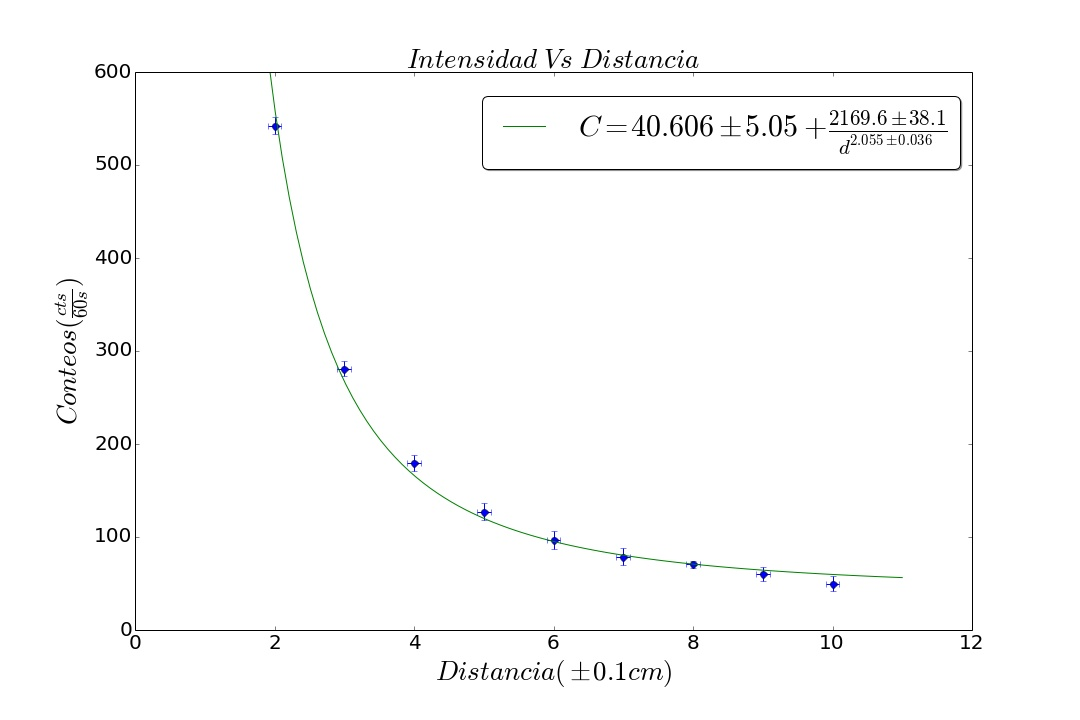
\includegraphics[width=1.1\linewidth]{distancia.jpg}
\caption{Relación de intensidad con la distancia a la fuente (Ra-226 débil)}
\label{fig:distancia}
\end{figure}

\begin{figure}[h!]
\centering
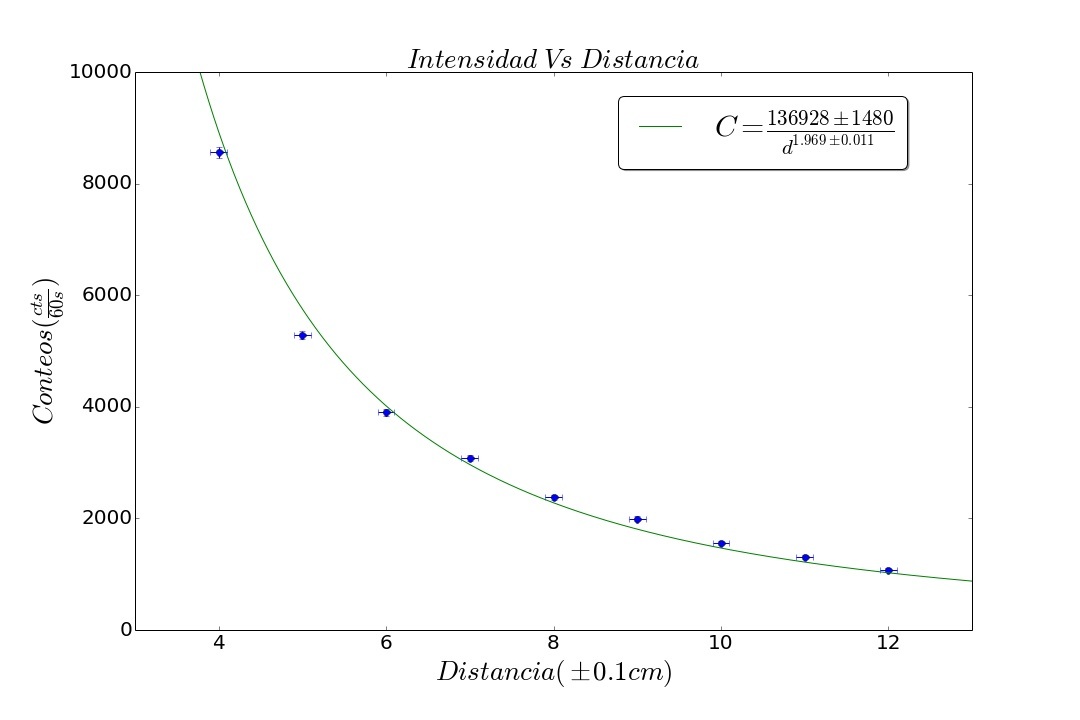
\includegraphics[width=1.1\linewidth]{cuadrados.jpg}
\caption{Relación de intensidad con la distancia a la fuente (Ra-226 fuerte)}
\label{fig:cuadrados}
\end{figure}

Dicho ajuste verifica la relación cuadrática de la intensidad con la distancia a la fuente. El valor del exponente es de $2.055\pm0.036$  para la fuente débil y de $1.969\pm0.011$ lo cual solo está alejado de la realidad un 2.75\% y un 1.5\%. La diferencias de errores se debe a la propagación de los errores relativos, los cuales son menores para conteos muy grandes.\\

Con esto concluimos que la intensidad de radiación decae inversamente con el cuadrado de la distancia a la fuente, independientemente de la fuente utilizada.\\
 
\subsection{\label{sec:level2}Rango de la radiación alpha}
En esta sección evaluamos el alcance de la radiación $\alpha$ emitida por una muestra de Ra-226. Para ello tomamos conteos durante 10 segundos variando la distancia sobre la muestra sin filtro, y la muestra con un filtro de papel. Los datos obtenidos se pueden apreciar en la tabla \ref{table:alcance}.\\

\begin{table}[h!]
\centering
 \begin{tabular}{|c|c|c|c|c|} 
 \hline
 $Distancia(\pm0.1cm)$& $C_{filtro}(\pm1)$& $\delta_{filtro}$ & $C_{0}(\pm1)$ & $\delta_0$ \\ [0.5ex] 
 \hline\hline
 3.00&5299&72.79&13640&116.79\\
 3.50&4225&65.00&11030&105.02\\
 4.00&3406&58.36&9570&97.83\\
 4.50&2722&52.17&7124&84.40\\
 5.00&2394&48.93&5740&75.76\\
 5.50&2106&45.89&4985&70.60\\
 6.00&1765&42.01&4230&65.04\\
 6.50&1558&39.47&3706&60.88\\
 7.00&1361&36.89&3163&56.24\\
 7.50&1159&34.04&2755&52.49\\
 8.00&1046&32.34&2500&50.00\\
 8.50&940&30.66&2258&47.52\\
 9.00&825&28.72&1989&44.60\\
 9.50&795&28.20&1841&42.91\\
 10.00&710&26.65&1652&40.64\\
 11.00&595&24.39&1369&37.00\\
 12.00&553&23.52&1098&33.14\\
 13.00&461&21.47&967&31.10\\
 14.00&334&18.28&818&28.60\\
 15.00&299&17.29&680&26.08\\
 16.00&288&16.97&582&24.12\\
 17.00&217&14.73&494&22.23\\
 18.00&205&14.32&417&20.42\\
 20.00&144&12.00&320&17.89\\
 25.00&97&9.85&189&13.75\\
 [1ex] 
 \hline
 \end{tabular}
 \caption{Mediciones de Ra-226 con y sin filtro de papel}
 \label{table:alcance}
\end{table}

Cabe resaltar que la fuente distanciatomada era sumamente radiactiva y para distancias muy cortas el contador se saturaba, por lo que se omitieron dichas medidas. Además, dado que no se tomaron muchas medidas se tomó como error absoluto la raiz cuadrada de las medidas, lo cual es una buena aproximación teniendo en cuenta la distribución de Poisson que caracteriza los decaimientos.\\

Ahora, para verificar el alcance de la radiación $\alpha$, tenemos que obtener en qué fracción se reduce la radiación total al imponer el filtro a diferentes distancias. Dicha fracción corresponde a la fracción  de rayos $\alpha$ en la radiación total. Cuando la fracción reducida sea significativamente pequeña, podemos decir que la radiación $\alpha$ llegó a su límite de distancia recorrida. En la tabla \ref{table:fraccion} se pueden apreciar las diferencias de radiación para cada distancia, así como la fracción que esta diferencia representa respecto a la radiación sin filtro. Los errores expuestos fueron calculados con la respectiva propagación de error tomando los errores de Poisson ya mencionados.\\ 

\begin{table}[h!]
\centering
 \begin{tabular}{|c|c|c|c|} 
 \hline
 $Distancia(\pm0.1cm)$& $\Delta C$& $Fraccion\ Reducida$ & $\delta_{frac}$ \\ [0.5ex] 
 \hline\hline
3.00&8341&0.612&0.006\\
3.50&6805&0.617&0.007\\
4.00&6164&0.644&0.007\\
4.50&4402&0.618&0.009\\
5.00&3346&0.583&0.010\\
5.50&2879&0.578&0.011\\
6.00&2465&0.583&0.012\\
6.50&2148&0.580&0.013\\
7.00&1802&0.570&0.014\\
7.50&1596&0.579&0.015\\
8.00&1454&0.582&0.015\\
8.50&1318&0.584&0.016\\
9.00&1164&0.585&0.017\\
9.50&1046&0.568&0.018\\
10.00&942&0.570&0.019\\
11.00&774&0.565&0.021\\
12.00&545&0.496&0.026\\
13.00&506&0.523&0.027\\
14.00&484&0.592&0.027\\
15.00&381&0.560&0.031\\
16.00&294&0.505&0.036\\
17.00&277&0.561&0.036\\
18.00&212&0.508&0.042\\
20.00&176&0.550&0.045\\
25.00&92&0.487&0.064\\
 [1ex] 
 \hline
 \end{tabular}
 \caption{Fracciones de reducción de radiación por el filtro}
 \label{table:fraccion}
\end{table}

En esta tabla se puede apreciar que la fracción de radiación $\alpha$ parada por el filtro de papel no varió significativamente en las distancias medidas. A pesar de esto si se pudo notar una disminución generalizada de esta radiación alrededor de los 5cm. Después de dicha distancia la fracción no varió generalizadamente. \\

Ahora, debido a la interacción del aire con la radiación $\alpha$, esta no tiene mucho alcance dependiendo de su energía. Para el aire a presión constante y a $15^oC$, este alcance está dado por $D= 0.4769 E^{1.5}\frac{cm}{Mev}$. Si tenemos en cuenta la caida en la fracción de radiación $\alpha$, podemos encontrar que la muestra emitía dichos rayos con energías alrededor de $4.80 MeV$. Con un poco de investigación podemos intuir que dicha energía corresponde a la transición $Ra-226 \rightarrow Ra-222$, la cual es de $4.871Mev$. Si esta es, en efecto, la transición correcta, este método de cálculo de energía provoca únicamente un $2\%$ de error, congruente con los errores obtenidos anteriormente con estos montajes.\\

\subsection{\label{sec:level2}Influencia del grosor de los materiales en la radiación $\beta$}
En este experimiento medimos la influencia del grosor de materiales como el cartón, perspex y aluminio sobre la radiación $\beta$ de una fuente de Ra-226. Para ello tomamos diferentes medidas de conteo durante 10 segundos con la muestra a 3 cm del detector. Los datos obtenidos se encuentran en las tablas \ref{table:carton}, \ref{table:perspex} y \ref{table:aluminio}.\\

\begin{table}[h!]
\centering
 \begin{tabular}{|c|c|c|c|c|c|} 
 \hline
 $Grosor(\pm0.1cm)$ & $c_1(\pm1)$ & $c_2(\pm1)$ & $c_3(\pm1)$ & $\bar{c}$ & $\sigma_c$ \\ [0.5ex] 
 \hline\hline
 0.0&9936&9824&9849&9869.67&48.00\\
 0.5&1467&1428&1482&1459.00&22.76\\
 1.0&697&664&739&700.00&30.69\\
 1.5&363&364&324&350.33&18.62\\
 2.0&211&199&219&209.67&8.22\\
 2.5&162&165&143&156.67&9.74\\
[1ex] 
 \hline
 \end{tabular}
 \caption{Filtros de aluminio de diferente grosor}
 \label{table:aluminio}
\end{table}

\begin{table}[h!]
\centering
 \begin{tabular}{|c|c|c|c|c|c|} 
 \hline
 $Grosor(\pm0.1cm)$ & $c_1(\pm1)$ & $c_2(\pm1)$ & $c_3(\pm1)$ & $\bar{c}$ & $\sigma_c$ \\ [0.5ex] 
 \hline\hline
 0.0&9193&9194&9081&9156.00&53.03\\
 1.4&1468&1462&1541&1490.33&35.91\\
 2.8&608&652&583&614.33&28.52\\
 4.2&358&350&398&368.67&21.00\\
 5.6&271&222&230&241.00&21.46\\
[1ex] 
 \hline
 \end{tabular}
 \caption{Filtros de perspex de diferente grosor}
 \label{table:perspex}
\end{table}

\begin{table}[h!]
\centering
 \begin{tabular}{|c|c|c|c|c|c|} 
 \hline
 $Grosor(\pm0.1cm)$ & $c(\pm1)$ & $\delta_c$ \\ [0.5ex] 
 \hline\hline
 0.0&9207&95.95\\
 1.5&4359&66.02\\
 3.0&2554&50.54\\
 4.5&1765&42.01\\
 6.0&1284&35.83\\
 7.5&791&28.12\\
 9.0&699&26.44\\
 10.5&557&23.60\\
[1ex] 
 \hline
 \end{tabular}
 \caption{Filtros de carton de diferente grosor}
 \label{table:carton}
\end{table}

En estos casos, como error absoluto de las medidas con filtros de aluminio y perspex, se utilizó la desviación estándar; sin embargo, para el cartón debido a sus grandes conteos por su bajo poder de filtro, se tomó solo una medida y su error fue obtenido como la raiz cuadrada del valor medido. \\

Ahora, la intensidad de radiación disminuye exponencialmente a través de un medio absorbente de la forma $I(d) = I_oe^{-\lambda d}$. Teniendo esto en cuenta, es necesario realizar un ajuste exponencial de esta forma, teniendo en cuenta la radiación ambiental como una constante aditiva. Dichos ajustes se encuentran representados en las figuras \ref{fig:aluminio}, \ref{fig:perspex} y \ref{fig:carton}.\\


\begin{figure}[h!]
\centering
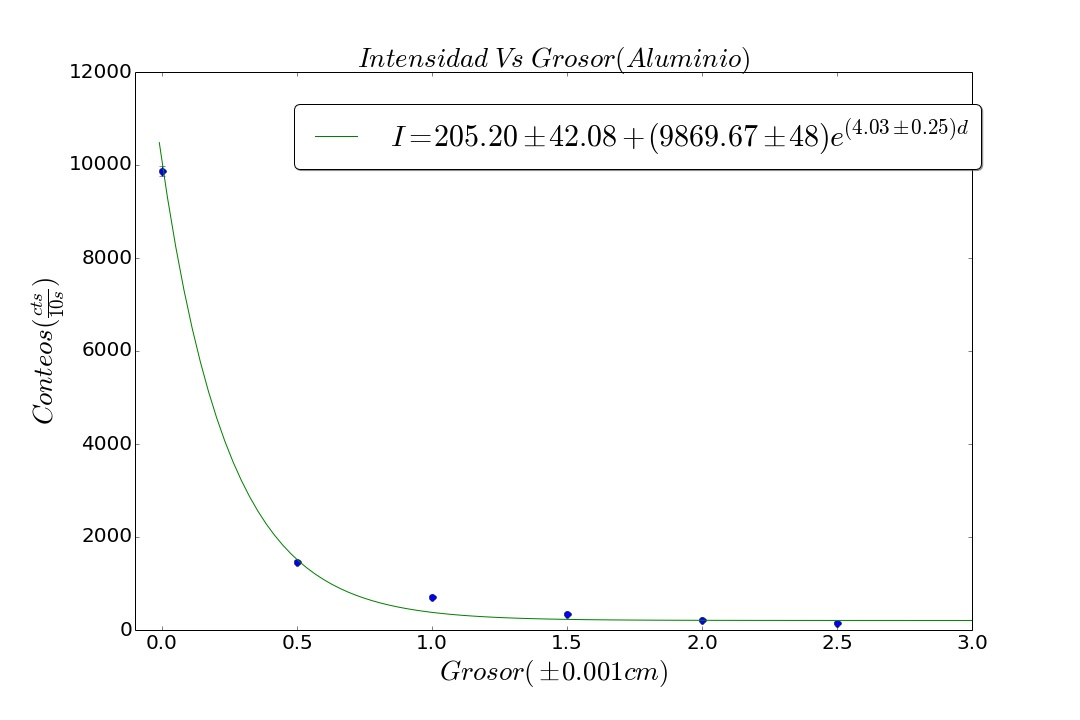
\includegraphics[width=1.1\linewidth]{aluminio.jpg}
\caption{Ajuste para la relació grosor-intensidad en el aluminio}
\label{fig:aluminio}
\end{figure}

\begin{figure}[h!]
\centering
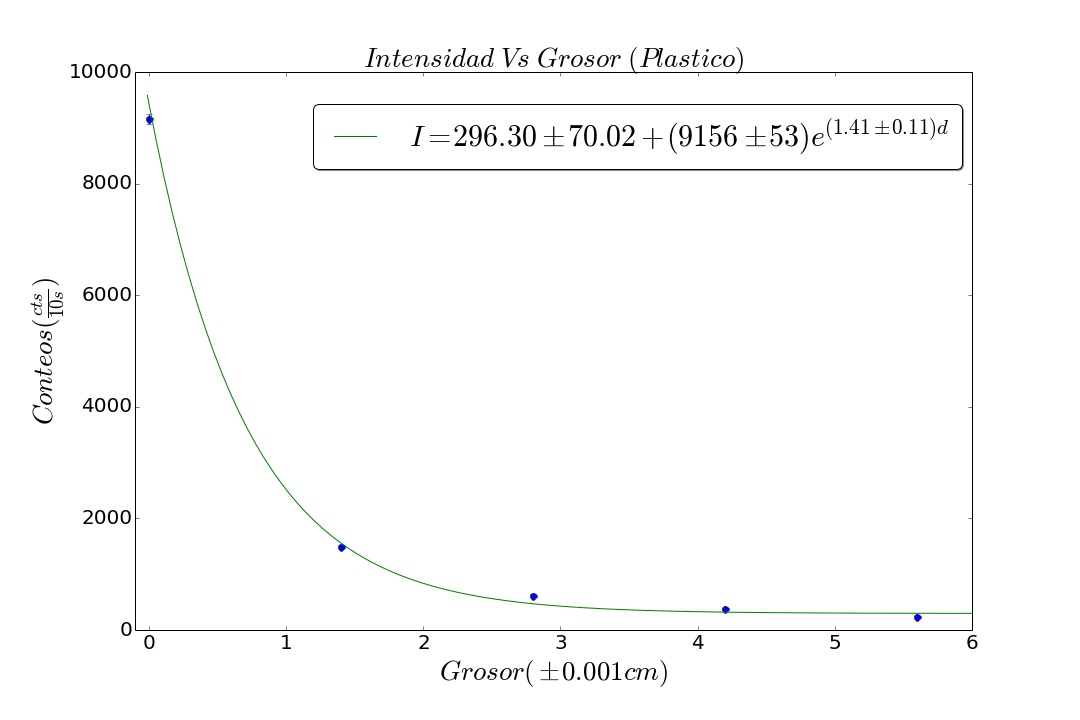
\includegraphics[width=1.1\linewidth]{perspex.jpg}
\caption{Ajuste para la relació grosor-intensidad en el perspex}
\label{fig:perspex}
\end{figure}

\begin{figure}[h!]
\centering
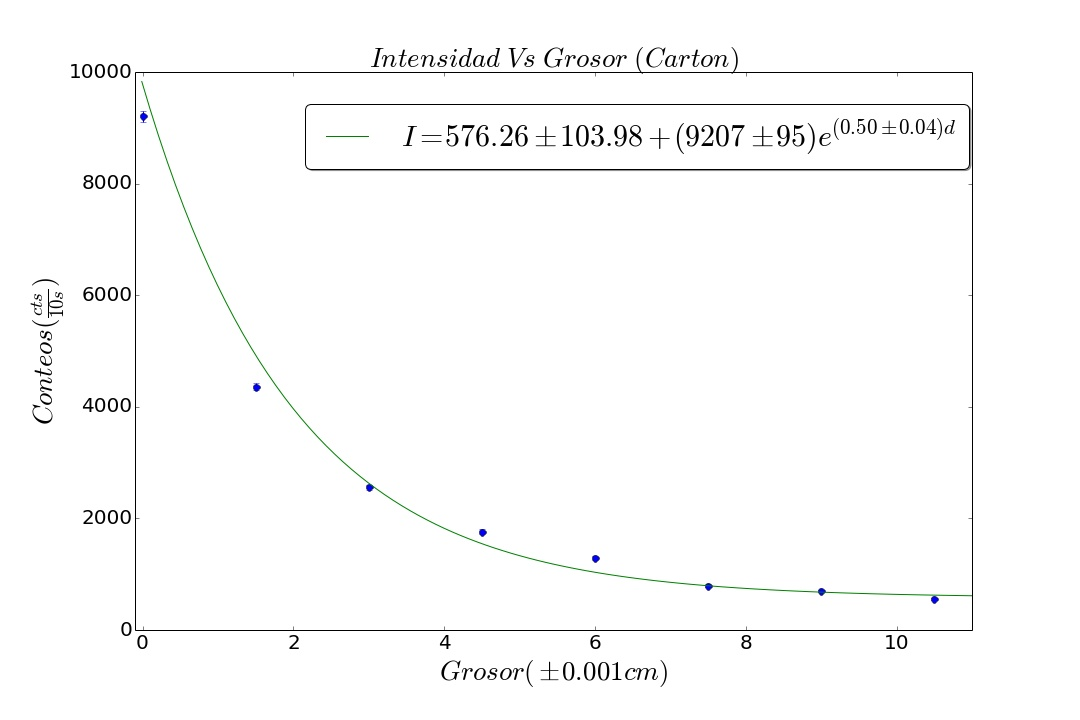
\includegraphics[width=1.1\linewidth]{carton.jpg}
\caption{Ajuste para la relació grosor-intensidad en el carton}
\label{fig:carton}
\end{figure}


En estas gráficas se puede apreciar que los coeficientes de absorción son respectivamente $\lambda_{al} = 4.04\pm0.25cm^{-1}$, $\lambda_{perspex} = 1.41\pm0.11cm^{-1}$ y $\lambda_{carton} = 0.50\pm0.04cm^{-1}$. El inverso de estos coeficientes nos darían una longitud de penetración para cada material, la cual es más intuitiva y más fácil de analizar. Dichas longitudes de penetración, con sus respectivos errores están dadas por: $d_{al} = 0.248\pm0.015cm$, $d_{perspex} = 0.709\pm0.055cm$ y $d_{carton} = 2.0\pm0.16cm$ .Así, según este indicador, el mejor filtro (entre los tres probados) para la radiación $\beta$ es el aluminio, seguido del perspex y luego del cartón.\\

\subsection{\label{sec:level2}Interacción de la radiación $\beta$ con campos magnéticos}
En este experimento no se pretendía tomar medidas, sino verificar cualitativamente la influencia de un campo magnético sobre la radiación $\beta$. Específicamente se quería ver cómo se deflectaba la radiación al imponer el mencionado campo magnético. Para esto, se tomaron medidas de conteo durante 10 segundos para ángulos de $0$ a $180^o$ equiespaciados a $10^o$ a una distancia de 8 cm con los magnetos, sin los magnetos y con los magnetos invertidos. Los datos tomados se encuentran en la tabla \ref{table:beta}.\\

Es preciso aclarar que hablamos únicamente de radiación $\beta$ dado que el único otro tipo de radiación que es cargada es la $\alpha$, la cual tiene el doble de carga que la radiación $\beta$ pero aproximadamente 8000 veces su masa, lo cual reduce el efecto de los campos magnéticos en un factor de aproximadamente 4000. En este sentido, el efecto del campo magnético solo será sobre la radiación $\beta$.\\

\begin{table}[h!]
\centering
 \begin{tabular}{|c|c|c|c|} 
 \hline
 $Angulo$& $Magnetos$ & $No Magnetos$ & $Magnetos Inv$ \\ [0.5ex] 
 \hline\hline
 0&221&300&200\\
10&201&366&247\\
20&166&430&306\\
30&180&730&466\\
40&303&1228&481\\
50&492&1582&689\\
60&707&1754&937\\
70&845&1544&1293\\
80&1051&1303&1533\\
90&1177&1153&1547\\
100&1299&976&1453\\
110&1444&753&1235\\
120&1652&652&932\\
130&1720&569&674\\
140&1505&473&527\\
150&941&299&447\\
160&602&193&362\\
170&479&180&288\\
180&383&209&215\\
[1ex] 
 \hline
 \end{tabular}
 \caption{Efecto del campo magnético en la radiación $\beta$}
 \label{table:beta}
\end{table} 

En esta tabla se puede notar que la intensidad de radiación tiende a concentrarse en $90^o$ cuando no hay magnetos involucrados. Esta dirección es la dirección de salida de los rayos producidos por el Ra-226 a través de su envoltura de plomo. Si se mira el efecto de los magnetos, en un caso la intensidad tiende a estar entre $0^o$ y $90^o$, y en el otro, su máximo tiende a concentrarse entre $90^o$ y $180^o$. Para entender este efecto de una mejor manera, se realizó una gráfica donde se mostraban los datos de la tabla anterior en un diagrama polar. En dicha figura \ref{fig:magneto}, en la escala angular se muestran los ángulos, y en la escala radial se grafica la intensidad.\\

\begin{figure}[h!]
\centering
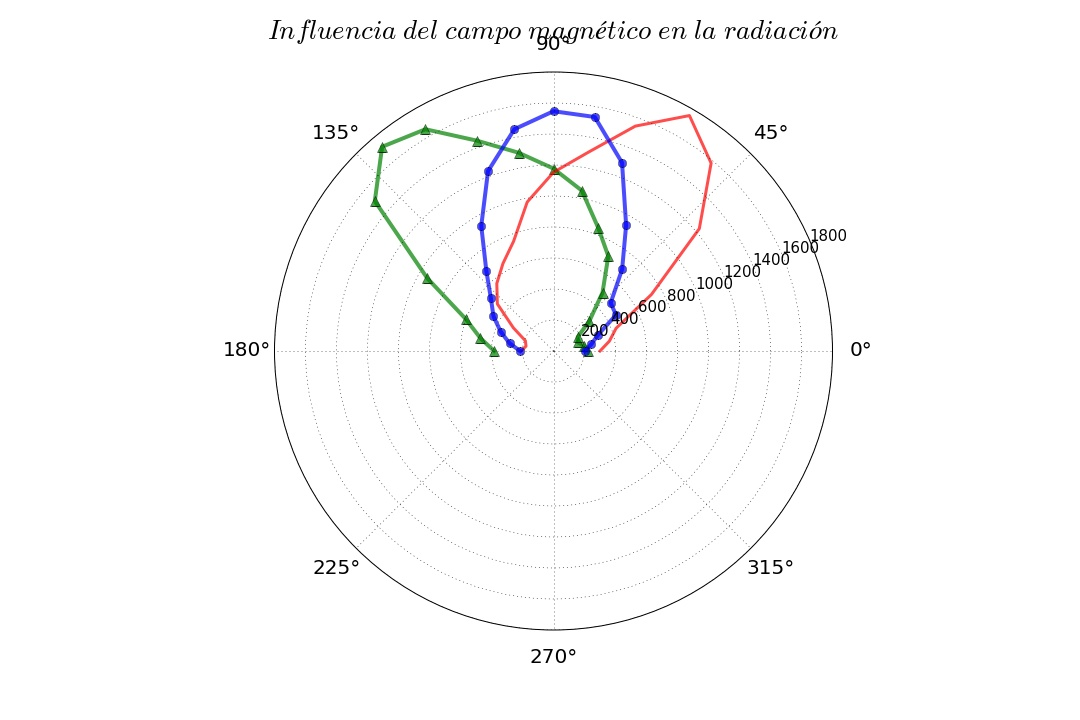
\includegraphics[width=1.1\linewidth]{magneto.jpg}
\caption{Influencia de los campos magnéticos sobre la radiación $\beta$}
\label{fig:magneto}
\end{figure}

En esta gráfica se puede apreciar que para el caso sin magnetos la función de intensidad es simétrica alrededor de su ángulo mayor, lo cual era de esperarse. Sin embargo, para los casos con magnetos, esta función de intensidad con respecto al ángulo tiende a rotar sin conservar la simetría alrededor de su máximo, favoreciendo el lado más cercano a la fuente de radiación ($90^o$). Esto puede ser explicad debido a los otros tipos de radiación que emite la muestra usada, $\alpha$ y $\gamma$, las cuales no se ven afectadas considerablemente por el campo magnético y por tanto se quedan en cerca a $90^o$. \\

\subsection{\label{sec:level2}Interacción de la radiación $\gamma$ con campos magnéticos}
Además de mostrar la influencia de los campos magnéticos sobre la radiación $\beta$, quisimos demostrar formalmente que estos campos no afectan la radiación $\gamma$. Para ello tomamos 4 medidas de 10 segundos con magnetos y sin ellos a la misma fuente radiactiva de Ra-226 cubierta siempre por una placa de aluminio. Los datos tomados con sus respectivos promedios y varianzas se encuentran en la tabla \ref{table:magplaca}.\\


\begin{table}[h!]
\centering
 \begin{tabular}{|c|c|c|} 
 \hline
 Medida & Magnetos & No-Magnetos \\ [0.5ex] 
 \hline\hline
 1&192&190\\
2&216&192\\
3&220&194\\
4&231&208\\
5&212&217\\
$\bar{c}$&214.2&200.2\\
$\sigma_c$&14.6&14.1\\
[1ex] 
 \hline
 \end{tabular}
 \caption{Efecto del campo magnético sobre la radiación $\gamma$}
 \label{table:magplaca}
\end{table}

En dicha tabla se puede observar que cada valor cae dentro del rango de incertidumbre del otro, lo cual nos dice que dadas dichas incertidumbres, los conteos son prácticamente iguales. De esta manera, la radiación $\gamma$ no se ve afectada por un campo magnético. La diferencia entre los promedios, sin tener en cuenta las varianzas, la podemos atribuir a que el aluminio no bloquea totalmente la radiación $\beta$ y un remanente de la radiación $\beta$ que si es deflectada, afecta la medida.\\

\subsection{\label{sec:level2}Tiempo de decaimiento}
En este montaje pretendíamos medir el tiempo de decaimiento del gas radiactivo que rodeaba a una manta incandescente. Para ello encerramos el gas en un recipiente y medimos 4 conteos consecutivos de 60 segundos. En este caso se trabajó con el aire que rodeaba a la manta debido a su poca densidad, lo cual permite un tiempo de decaimiento más corto, observable con estos montajes. En este sentido, dicho aire es poco radiactivo y el efecto del ambiente juega un papel importante, por lo cual también fue medido. Las tablas con los datos obtenidos son \ref{table:decambiente} y \ref{table:decaire}.\\

\begin{table}[h!]
\centering
 \begin{tabular}{|c|c|c|} 
 \hline
 Medida & Ambiente \\ [0.5ex] 
 \hline\hline
 1&12\\
 2&17\\
 3&19\\
 4&26\\
 $\bar{c}$&18.5\\
 $sigma_c$&4.3\\
[1ex] 
 \hline
 \end{tabular}
 \caption{Radiación ambiente (Tiempo de decaimiento)}
 \label{table:decambiente}
\end{table}

\begin{table}[h!]
\centering
 \begin{tabular}{|c|c|c|} 
 \hline
 Tiempo & $c$ & $\sigma_c$\\ [0.5ex] 
 \hline\hline
 60&60&7.75\\
 120&43&6.56\\
 180&32&5.66\\
 240&27&5.20\\
[1ex] 
 \hline
 \end{tabular}
 \caption{Decaimiento de radiación del aire radiactivo}
 \label{table:decaire}
\end{table}

En estos casos se puede apreciar que claramente los conteos del aire radiactivo disminuian con el tiempo que pasaba. Ahora, la ley de decaimiento, dada por la ecuación \ref{eq:tiempo} nos permite obtener un ajuste exponencial teniendo en cuenta que se tiene que restar la radiación del ambiente. Dicho ajuste se encuentra en la figura \ref{fig:deca}.\\

\begin{equation}
I(t) = I_0 e^{\frac{t}{\tau}}
\label{eq:tiempo}
\end{equation}

\begin{figure}[h!]
\centering
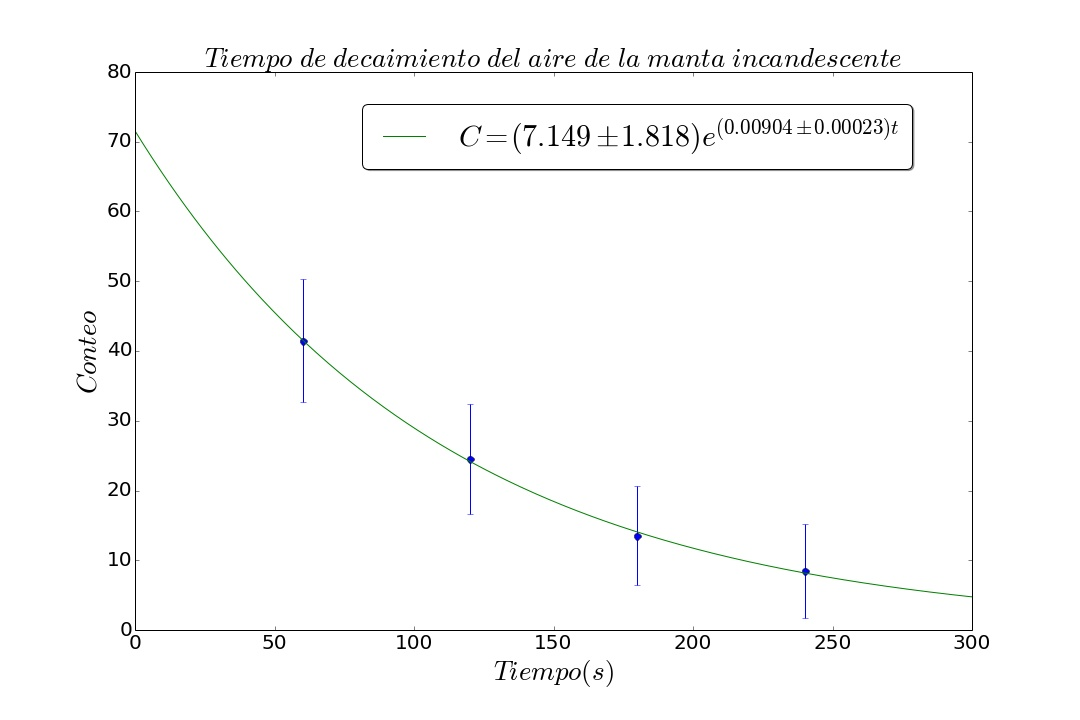
\includegraphics[width=1.1\linewidth]{decaimiento.jpg}
\caption{Tiempo de decaimiento del aire que rodea una manta incandescente}
\label{fig:deca}
\end{figure}

De esta gráfica se puede notar que el ajuste es muy preciso y arroja un tiempo de decaimiento de $0.00904\pm0.00023s^{-1}$, lo cual, en otras palabras nos dice que el aire que rodea la manta tiene un tiempo de decaimiento de 110 segundos, justamente observable en este experimento. A pesar de la propagación de error por la medida del ambiente y la propia medida del aire radiactivo, el error relativo de este ajuste fue de aproximadamente 2.5\%, el error relativo usual asociado a este montaje.\\


\section{\label{sec:level1}Conclusiones}
Una de las conclusiones más importantes de este experimento, la cual estuvimos utilizando durante todo el análisis numérico, fue la definición de la distribución de probabilidad que rige los decaimientos radiactivos. Dicha distribución es de Poisson y esto nos da el poder para deducir valores de varianza sin tener muestras estadísticas significativamente grandes.\\

Además de esto, verificamos que la radiación ionizante se compone de los 3 tipos $\alpha$, $\beta$ y $\gamma$, los cuales se pueden clasificar de acuerdo a su poder de penetración. De estos tipos de radiación descubrimos que los rayos $\beta$ son cargados con masa pequeña y que los rayos $\gamma$ no tienen carga. Sobre los rayos $\alpha$ no hicimos experimentos explícitos con campos magnéticos, pero pudimos verificar que estos, a comparación de los rayos  $\beta$, no se ven afectados por campos magnéticos pequeños debido a su gran masa.\\

Descubrimos que algunas sales que son en principio no radiantes, tienen trazas de isótopos radiactivos que hacen que emitan radiación ionizante detectable con los montajes propuestos.\\

Pudimos verificar además, con alrededor de 2\% de precisión, que la intensidad de radiación disminuía como el inverso de la distancia de la fuente al cuadrado y como una ley exponencial al penetrar cierta distancia en un material absorbente.\\

Los errores obtenidos fueron muy similares porque debido a la propagación de error de las medidas tomadas. Dicho error dependía del tamaño del conteo realizado y debido a que en muchos experimentos se usó el Ra-226, dichos conteos eran muy similares.\\

En general, a pesar de la estocasticidad natural de cada experimento, se pudieron obtener resultados concretos con muy buena exactitud.\\




\begin{thebibliography}{99} 
\bibitem{Griffiths} David J. Griffiths,{\it Introduction to electrodynamics 4Ed.}\\ 
\bibitem{guia} ,{\it Instruction Manual and Experiment Guide for the PASCO scientific Model WA-9314B}{1991}.\\ 
\end{thebibliography}




\end{document}
%
% ****** End of file apssamp.tex ******
